%!TEX root = Thesis.tex
                                            
\section{Effective Probabilistic Simulation}\label{sec:ProbSimu}


  The final refinement performs a full-circuit stochastic simulation. Although we obtain a set of potential design variables from Section~\ref{sec:reTarg}, these do not represent the optimal solution. The final refinement performs simulation to prevent the solution from any non-ideal effects via higher-level abstraction. After {\it Design Re-targeting}, a set of overall device level variable values $\Psi $ are collected. $N_{V^D}$ collects the number of all device variables type. Since these design variables are selected by performance exploration via transformation, each population of performance metrics directly projects to a set of variable distribution. Basically, $\Psi$ provides the variable space for perturbation. By swapping among device-level parameters, the cost of full-circuit simulation is reduced. By employing global optimization algorithm, such as random walk or simulated annealing, the entire circuit is re-constructed and fed into circuit simulator using real models and parameters from the foundry.

  \begin{figure}[ht]
      \centering
      \begin{subfigure}[t]{0.4\textwidth}
        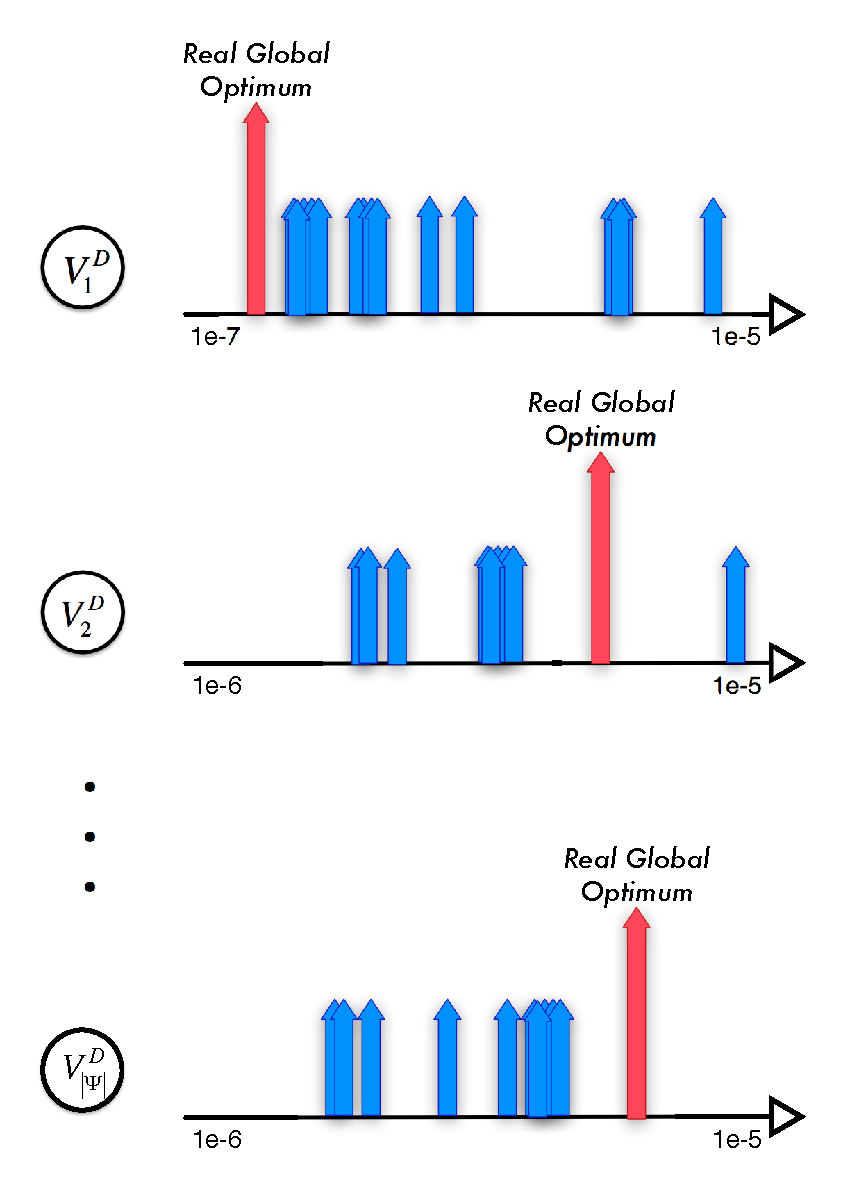
\includegraphics[width=\textwidth]{Fig/Chapter2/popSampling.eps}
      \end{subfigure}
      \begin{subfigure}[t]{0.4\textwidth}
        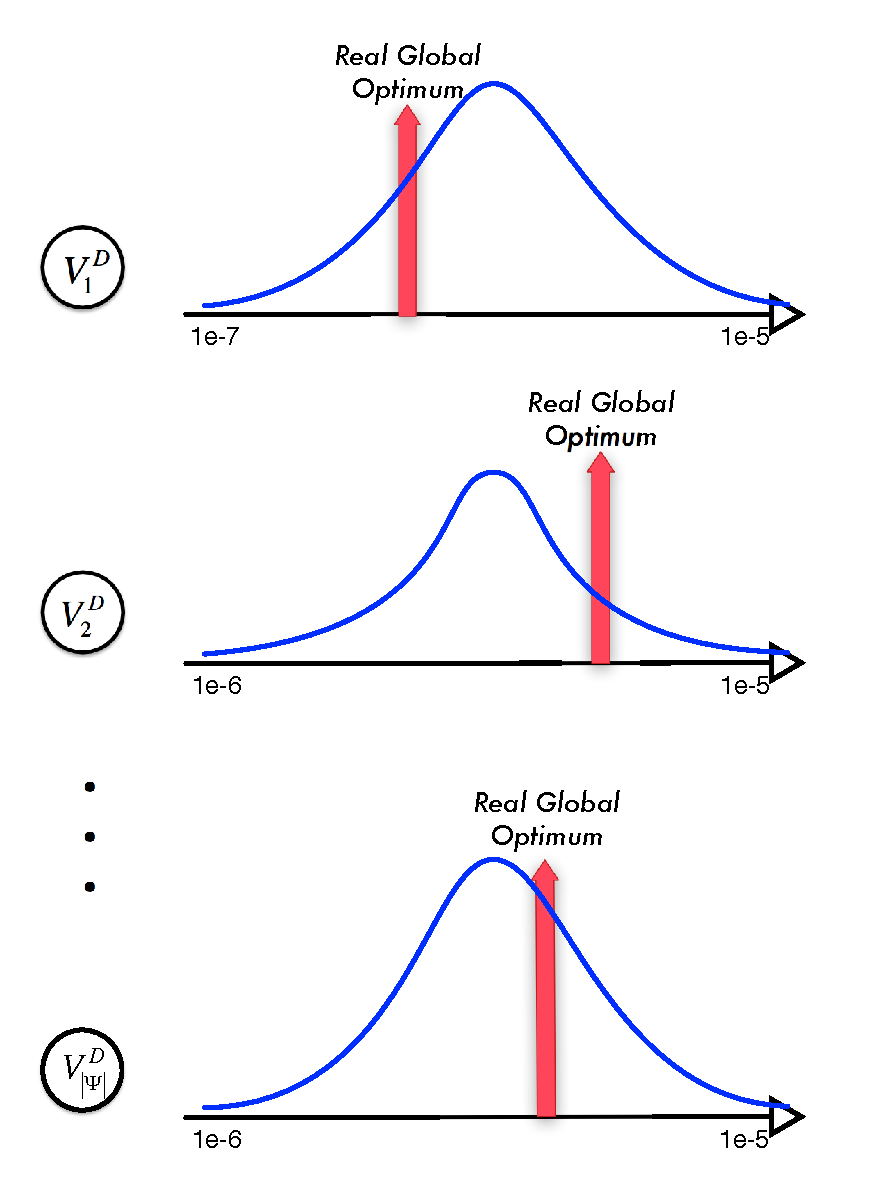
\includegraphics[width=\textwidth]{Fig/Chapter2/norPopDis.eps}
      \end{subfigure}
      \caption
      {
        Different distribution for stochastic simulation. (a) Population samplings for each device level variable from population and the global optimum location. (b) Normal distributions for each device level variable after normalized and the global optimum location.
      }\label{fig:optimumValleys}
  \end{figure}

  Such multi-objective simulated annealing (SA) based stochastic simulation is implemented in \cite{PerfMap_ISQED2011}. During perturbation, each swap of $V^D_m$ is referred to a uniform manufacturable range with respect to each device variable ($V^D_{M_{min}},V^D_{M_{MAX}}$). Since the range of each device variable is uncertain and continuous, the solution set can be wide. Normally, a movement among the range of $V^D_M$ is decided by the uniform probability, i.e., every movement is randomly chosen in the equal chance. As a matter of fact, some corner values are trivially unfeasible, and it is time-consuming to evaluate unfeasible solutions. Even if multi-objective SA has a good initial solution, the full range stochastic simulation accompanies with vast computing time to converge. We observe that the perturbation strategy can be performed statistically. 
    

  To ease the effort with simulation, the possibility of each movement among the range of $V^D_M$ can be manipulated. For each $V^D_M$, $N_P$ samples are collected via {\it Design Re-targeting}. Therefore, these samples construct a distribution for $V^D_M$. Since all of them are potential candidates for optimal solution, We believe that the sparser density results in less likelihood toward optimal solution. Consequently, the distribution of $V^D_M$ forecasts the performance behaviors related to probability. To extend this idea, the distribution of $V^D_M$ values can be transferred into the probability density function (PDF) and cumulative distribution function (CDF), and every movement of swap is determined by such function. Different from the uniform manufacturable range, it is closer to the behavior of performance metrics. Theoretically, the global optimum oughts to among these peaks of distributions with respect to each device variable. Roughly, performance results are quite close to real circuit simulation results such as SPICE. In other words, every prediction result from genetic based performance exploration projects to a device variable set, and the PDF-deterministic perturbation for circuit simulation benefits the convergence of multi-objective optima performance.


  \newcommand{\PFTS}{\ensuremath{\mbox{\sc ProbFineTuneSimulation}}}
  \algloopdefx{RETURN}[1][]{\textbf{return} #1}
  \algblockdefx{FORALLP}{ENDFAP}[1]%
    {\textbf{for all }#1 \textbf{do in parallel}}%
    {\textbf{end for}}
  \begin{algorithm}[ht]  
    \caption{$\PFTS(T,T_{freeze}, \Psi, r, N_s)$}\label{alg:PFTS}                       
    \begin{scriptsize}
      \begin{algorithmic}[1]
        \REQUIRE 
          \begin{tabular}{l}
            $T$: A initial temperature, $T>0$.\\
            $T_{freeze}$: Frozen temperature for annealing.\\
            $\Psi$: A set of overall device parameter values.\\
            $r$: A factor to reduce temperature T.\\
            $N_s$: Number of normal distribution sampling.\\
          \end{tabular}
        \ENSURE
          \begin{tabular}{l}
            $\hat{V^D_M}$: Optimal design parameters. \\
            $R$: Optimal performance data from simulation. \\
          \end{tabular}
        \FOR {$j = 1 \to |M|$}
          \STATE $mean_j=CalculateMean(\Psi,j)$
          \STATE $std_j=CalculateVariance(\Psi,j)$
          \STATE $pdf_{j}=normalPDFGenerator(mean_j, std_j,N_s)$
        \ENDFOR
        \FOR{$j= 1 \to |M|$}
          \STATE $V^D_{m_j} = mean_j$
        \ENDFOR
        \STATE $R=Evaluate(V^D_M),\; V^D_M = \{V^D_{m_j}| 1 \leq j \leq |M|\}$
        \WHILE {$T > T_{freeze}$}
          \FOR {$j = 1 \to |M|$}
            \STATE ${V^D_{m_j}}' = Move(pdf_j)$
          \ENDFOR
          \STATE $R'=Evaluate({V^D_M}')$
          \IF{$cost(R') \prec cost(R)$}
            \STATE $R' \gets R$
          \ELSE
            \STATE $R' \gets R\ with\ probability\ min(1,exp\{ -\frac{\delta E(cost(R'),cost(R)} {T}\})$
          \ENDIF
          \STATE $T \gets rT$
        \ENDWHILE
          \STATE $\hat{V^D_M} \gets V^D_M$
        \STATE $return\ R$          
      \end{algorithmic}
    \end{scriptsize} 
  \end{algorithm}

  As illustrated in Fig.~\ref{fig:optimumValleys} (a), while swapping according to the distribution of $V^D_M$, discrete distribution affects the accuracy of movement schedule. In addition, the original distribution is refurbished as normalized distribution. Later, the normal distribution for each device variable $V^D_M$ is obtained (shown in Fig.~\ref{fig:optimumValleys} (b)). The nearest point to the mean value from samples symbolizes higher potential to reach the global optimum. Also, the normal distribution ensures that the probability of every movement manufacturable range is feasible. On the boundary of such distribution, the probability decreases and results in less visiting while swapping. Regarding the uniform simulation, since all of samplings have equal probability, SA based simulation spends more efforts on local solution. Other than the uniform approach, this strategy forbids certain trivial simulation with worse performance.  


  In detailed implementation (shown in Algorithm~\ref{alg:PFTS}), given the variable sets, normalized distributions for each design variable are generated by calculating the mean values and standard deviations. In other words, it represents the probability density function (PDF) for that device-level variable. The Box-Muller method \cite{BoxMuller1958AMS} uses two independent random number, then it generates two standard normal distribution variables. As Eq.(\ref{eq:BoxMullerEq}) illustrated, two independent random numbers $U$ and $V$ are distributed uniformly between (0,1), then the two standard normal distribution variables $X$ and $Y$ are generated. two normal distribution variables $X'$ and $Y'$ are further obtained in terms of $\mu$ and $\sigma^2$ ($\mu$ is the mean and $\sigma^2$ is the variance). A set of PDF for each device-level variable is generated after dividing all of samplings into several intervals and calculate the number of interval sampling to get the PDF from $\Psi$. $PDF = \{ {pdf}_k | 1 \leq k \leq |M|\}$.
    

  \begin{align}{\label{eq:BoxMullerEq}}
    \begin{array}{l}
      \exists \ U\sim\mathcal{U}(0,1)\ and\ V\sim\mathcal{U}(0,1)\\
      \Rightarrow \left\{
      \begin{array}{l}
      %X=R\cos(\theta)\\
      %Y=R\sin(\theta)\\
        X=\sqrt{-2lnU}\cos(2\pi V)\\
        Y=\sqrt{-2lnU}\sin(2\pi V)\\
      \end{array}
      \right .
      X,\ Y\sim\mathcal{N}(0,1)\\
      Extend:\\
      \left\{
      \begin{array}{l}
        X'=\sqrt{-2lnU}\cos(2\pi V)\times \sigma+\mu\\
        Y'=\sqrt{-2lnU}\sin(2\pi V)\times \sigma+\mu\\
      \end{array}
      \right .
      X,\ Y\sim\mathcal{N}(\mu,\sigma^2)\\
    \end{array}
  \end{align} 

  


  We assign maximum and minimum values for each $V^D_m$ from technology design rules, and then apply {\it Probabilistic Perturbation Fine Tuning} among these variable boundaries based on multi-objective perturbation as shown in Algorithm~\ref{alg:PFTS}. The $normalPDFGenerator$ use Box-Muller method to generate PDF for each $V^D_M$ is shown in Algorithm~\ref{alg:normalPDFGenerator}.


  From Line 1 to Line 5 in Algorithm~\ref{alg:PFTS}, it illustrates the PDF generates process for each device variable $V^D_m$. Before multi-objective perturbation, the initial solution is selected. According to the PDF function for each $V^D_m$, the mean value represents a good initial point for simulation (from Lin 6 to Line 8). Thus, we obtain the the initial solution $R$ via $Evaluate(V^D_M)$ in Line 9. Later, it proposes the multi-objective SA to converge the optimal solution from Line 10 to Line 22. Originally, the $Move(pdf)$ function selects a point between $V^{D}_{m_{max}}$ to $V^{D}_{m_{min}}$ randomly. However, this kind of selection picks up the optimal value and the corner value of variable $V^D_m$ with the equal probability. To leverage the distribution of each variable $V^D_m$, we try to select next $V^D_m$ value according to different possibility. Therefore, $Move(pdf_j)$ selects value of each $V^D_m$ accord to $pdf_j$ generated by Algorithm~\ref{alg:normalPDFGenerator}. Fig.~\ref{fig:NorPDFSwap} demonstrates one example of $Move(pdf_j)$ operation. In Algorithm~\ref{alg:PFTS} Line 14, the set of device variables ${V^D_M}'$ is fed into circuit simulator to obtain result $R'$. If $R'$ dominates $R$ (or $R' \prec R$), the new solution $R'$ is accepted. The dominant relationship is defined in {\it Definition~\ref{def:Dominate}}. For the objective function in {\it Definition~\ref{def:Dominate}},we apply a composite function method to obtain the combined cost function of multi-objective values in {\it Definition~\ref{def:objective}} which is inspired by Engrand et al.~\cite{EngrandMOSA}. While $R'$ does not dominate $R$, it still has probability to accept $R$ (shown in Algorithm~\ref{alg:PFTS} Line 18) and then the temperature $T$ is cooled down factor $r$. $ProbFineTuneSimulation$ terminates when the temperature $T$ reaches $T_{freeze}$ then an optimal result $R$ is achieved.


  \newcommand{\normalPDFGenerator}{\ensuremath{\mbox{\sc normalPDFGenerator}}}
  \algloopdefx{RETURN}[1][]{\textbf{return} #1}
  \algblockdefx{FORALLP}{ENDFAP}[1]%
  {\textbf{for all }#1 \textbf{do in parallel}}%
  {\textbf{end for}}
  \begin{algorithm}[t]  
    \caption{$\normalPDFGenerator(M, Std, N_s)$}\label{alg:normalPDFGenerator}                       
    \begin{scriptsize}
      \begin{algorithmic}[1]
        \REQUIRE 
        \begin{tabular}{l}
          $M$: Mean of population sampling.\\
          $Std$: Standard deviation of population sampling.\\
          $N_{total}$: Number of Box-Muller method sampling.\\
        \end{tabular} 
        \FOR {$j = 1 \to N_{total}$}
          \STATE $U=rand(0,1)$
          \STATE $V=rand(0,1)$
          \STATE $X=\sqrt{-2lnU}\cos(2\pi V)\times Std + M$
          \STATE $Y=\sqrt{-2lnU}\sin(2\pi V)\times Std + M$
        \ENDFOR
        \STATE $Z\gets X, Y$
        \FOR {$i = 1 \to N_s$}
          \STATE $pdf_{i}\gets \frac{NumberOfSampling(Z, i, i-1)}{N_{total}}$
        \ENDFOR
        \STATE $return\ pdf$
      \end{algorithmic}
    \end{scriptsize} 
  \end{algorithm}

  \begin{figure}[ht]
    \centering
    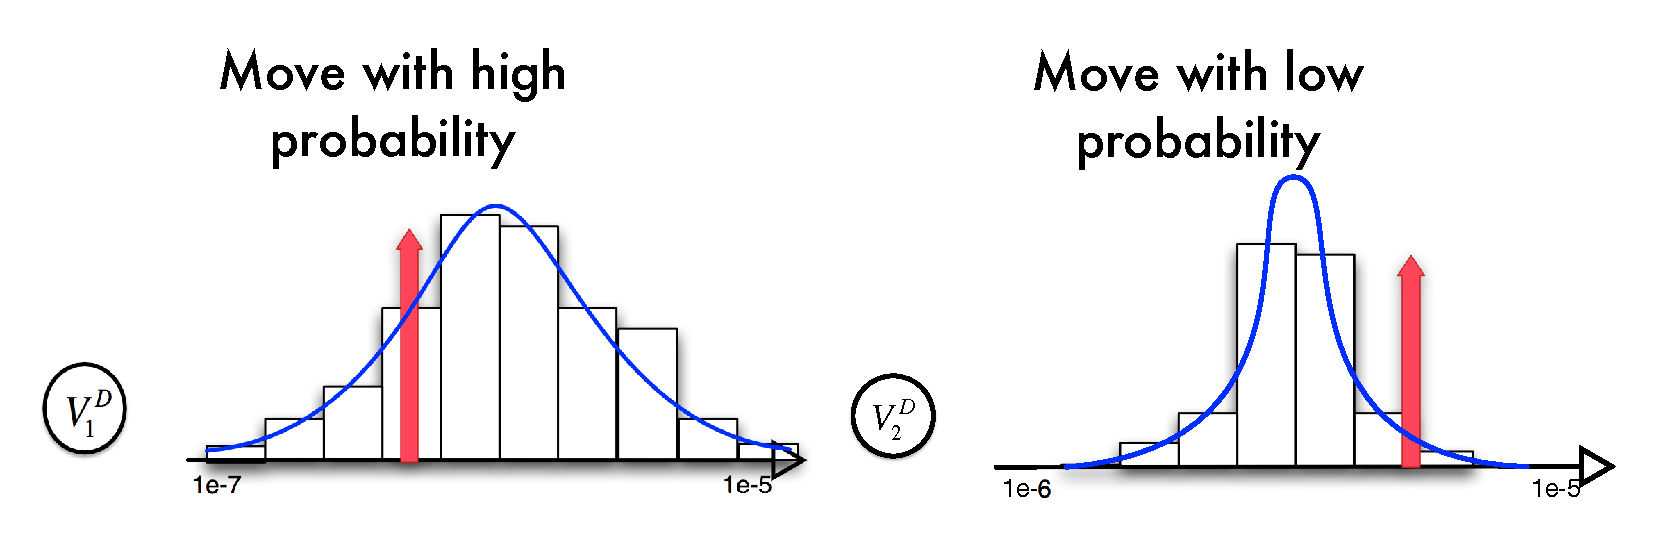
\includegraphics[width=0.7\textwidth]{Fig/NorPDFSwap.eps}
    \caption{Swap behavior dominated by probabilistic in PDF of $V^D_m$} 
    \label{fig:NorPDFSwap}
  \end{figure}


  \newtheorem{PFTSDef}{Definition}
  %\newtheorem{Dominate}[func]{Definition}
  \begin{defi}\label{def:Dominate}
    x $\prec$ y (called x dominates y) iff $E_i(x)$ $\leq$ $E_i(y)$, for i=1,\dots ,K and $E_j(x)$ $\leq$ $E_j(y)$ for least one objective function $E_j$.
  \end{defi}

  \begin{defi}\label{def:objective}
    The composite objective function is defined, $E=\displaystyle\sum_{n=1}^{K} ln(w_if_i(x))$, where $f_1$, $\dots$ ,$f_K$ are K objectives to be optimized and $w_i$ is normalized weighting value corresponding to each objective result, for i=1, $\dots$ ,k.
  \end{defi}

